% ============================================================
%  Příprava na maturitu – Elektrotechnika
%  Okruh 16: AD a DA převodníky
% ============================================================

\documentclass[a4paper,10pt]{article}

\usepackage[T1]{fontenc}
\usepackage[utf8]{inputenc}
\usepackage[left=2.0cm, right=1.8cm, top=1.8cm, bottom=1.8cm]{geometry}
\usepackage{parskip}
\usepackage{xcolor}
\usepackage{tabularx}
\usepackage{booktabs}
\usepackage{tikz}
\usepackage{mdframed}
\usepackage{amsmath}
\usepackage{enumitem}
\usepackage{circuitikz}

\usetikzlibrary{arrows.meta, positioning, decorations.pathmorphing, shapes.geometric, calc}

% --- Barvy ---
\definecolor{accent}{HTML}{1A3A5C}
\definecolor{lightblue}{HTML}{EAF2F8}
\definecolor{lightyellow}{HTML}{FDFBE4}
\definecolor{lightgreen}{HTML}{EAF7EA}
\definecolor{lightred}{HTML}{FDE8E8}
\definecolor{lightgray}{HTML}{F4F4F4}

% --- Boxy ---
\newmdenv[backgroundcolor=lightblue,linecolor=accent!40,roundcorner=4pt,
  innertopmargin=6pt,innerbottommargin=6pt,innerleftmargin=8pt,innerrightmargin=8pt]{pojmybox}
\newmdenv[backgroundcolor=lightyellow,linecolor=accent!30,roundcorner=4pt,
  innertopmargin=6pt,innerbottommargin=6pt,innerleftmargin=8pt,innerrightmargin=8pt]{vysvetlenibox}
\newmdenv[backgroundcolor=lightgreen,linecolor=accent!40,roundcorner=4pt,
  innertopmargin=6pt,innerbottommargin=6pt,innerleftmargin=8pt,innerrightmargin=8pt]{vzorcebox}
\newmdenv[backgroundcolor=lightred,linecolor=accent!30,roundcorner=4pt,
  innertopmargin=6pt,innerbottommargin=6pt,innerleftmargin=8pt,innerrightmargin=8pt]{durazbox}

\setlist[itemize]{noitemsep, leftmargin=1.4em, topsep=2pt}
\setlist[enumerate]{noitemsep, leftmargin=1.4em, topsep=2pt}

% --- Zkratka pro jednotky ---
\newcommand{\jednotka}[1]{\,[\mathrm{#1}]}

\begin{document}

% ============================================================
\section*{\large Okruh 16 – AD a DA převodníky}

\begin{pojmybox}
\textbf{Klíčové pojmy:}
spojitý a diskrétní signál, vzorkování, Shannon-Kotělnikovův teorém, kvantování, kódování, rozlišení (bity), D/A převodník, síť R-2R, A/D převodník paralelní (Flash), s postupnou aproximací (SAR), integrační
\end{pojmybox}

\begin{vysvetlenibox}

% ================================================================
\subsection*{1. Analogový vs. Číslicový signál}

\begin{itemize}
    \item \textbf{Analogový (Spojitý) signál:} Může nabývat nekonečně mnoha hodnot v čase i amplitudě (např. teplota, zvuk z mikrofonu).
    \item \textbf{Číslicový (Diskrétní) signál:} Je definován jen v určitých časových okamžicích a může nabývat pouze omezeného počtu přesně daných hodnot (logická 0 a 1).
\end{itemize}

% ================================================================
\subsection*{2. Proces A/D převodu (Analog $\to$ Digital)}

Převod spojitého signálu do procesoru probíhá ve třech krocích:

\begin{enumerate}
    \item \textbf{Vzorkování (Sampling):} Z analogového signálu se v pravidelných intervalech (vzorkovací frekvence $f_{vz}$) odebírají aktuální hodnoty napětí.
    \item \textbf{Kvantování (Quantization):} Naměřená hodnota se zaokrouhlí na nejbližší povolenou úroveň napětí (podle rozlišení převodníku). Vzniká tzv. kvantovací chyba (šum).
    \item \textbf{Kódování (Coding):} Zjištěné úrovni se přiřadí binární číslo (např. 10110011), které se pošle do počítače.
\end{enumerate}

\begin{center}
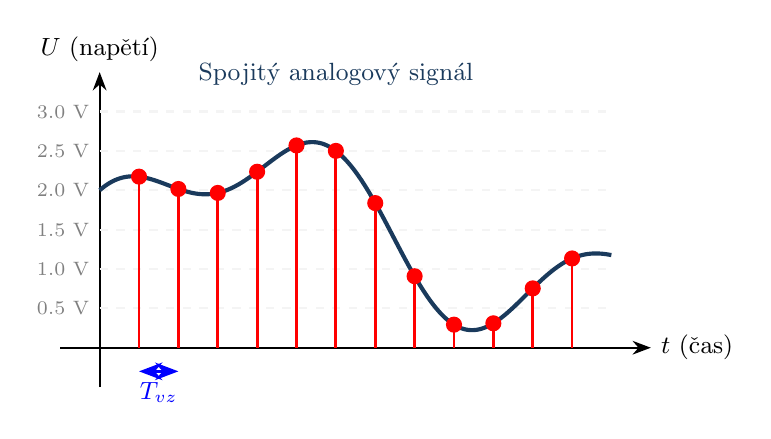
\begin{tikzpicture}[>=Stealth, font=\small, thick]
  % Osy
  \draw[->] (-0.5,0) -- (7,0) node[right] {$t$ (čas)};
  \draw[->] (0,-0.5) -- (0,3.5) node[above] {$U$ (napětí)};

  % Kvantizační úrovně (horizontální linky)
  \foreach \y in {0.5, 1.0, 1.5, 2.0, 2.5, 3.0} {
    \draw[dashed, lightgray] (0,\y) -- (6.5,\y);
    \node[left, font=\scriptsize, gray] at (0,\y) {$\y$ V};
  }

  % Definice matematické funkce signálu pro přesné lícování bodů
  \tikzset{declare function={f(\x)=1.5 + sin(\x*50) + 0.5*cos(\x*120);}}

  % Spojitý signál vykreslený pomocí definované funkce
  \draw[accent, line width=1.5pt, smooth, samples=100, domain=0:6.5] plot (\x, {f(\x)});
  \node[accent, above] at (3, 3.2) {Spojitý analogový signál};

  % Vzorky (červené body) PŘESNĚ ležící na křivce f(x)
  \foreach \x in {0.5, 1.0, 1.5, 2.0, 2.5, 3.0, 3.5, 4.0, 4.5, 5.0, 5.5, 6.0} {
    \draw[red, line width=1pt] (\x,0) -- (\x,{f(\x)});
    \filldraw[red] (\x,{f(\x)}) circle (2.5pt);
  }

  % Vzorkovací perioda
  \draw[<->, blue, line width=1.2pt] (0.5, -0.3) -- (1.0, -0.3) node[midway, below] {$T_{vz}$};
\end{tikzpicture}
\end{center}

\begin{durazbox}
\textbf{Shannon-Kotělnikovův teorém:}
Aby bylo možné z digitálních dat zpětně a bez zkreslení zrekonstruovat původní analogový signál, musí být vzorkovací frekvence ($f_{vz}$) \textbf{minimálně dvakrát vyšší} než nejvyšší frekvence obsažená v měřeném signálu ($f_{max}$).
\[
f_{vz} \ge 2 \cdot f_{max}
\]
\textit{Příklad: Lidské ucho slyší do 20\,kHz. Proto se hudba na CD vzorkuje frekvencí 44,1\,kHz (což je s rezervou více než $2 \cdot 20$).}
\end{durazbox}

% ================================================================
\subsection*{3. Parametry převodníků}

Základním parametrem je \textbf{Rozlišení $n$ (počet bitů)}. Určuje, na kolik "schodečků" (úrovní) dokáže převodník rozdělit měřený rozsah napětí.
Počet úrovní $N = 2^n$.

\begin{vzorcebox}
\[
\text{Krok převodníku (LSB)} = \frac{U_{ref}}{2^n}
\]
\end{vzorcebox}
\textit{Příklad: 10bitový převodník (dnes běžný v mikrokontrolérech) má $2^{10} = 1024$ úrovní. Pokud měří rozsah 0--5\,V, dokáže rozeznat změnu napětí (jeden krok) o velikosti $5\,\mathrm{V} / 1024 \approx 4{,}88\,\mathrm{mV}$.}

% ================================================================
\subsection*{4. D/A Převodníky (Digital $\to$ Analog)}

Vytvářejí analogové napětí na základě přivedeného binárního čísla.

\textbf{Převodník se sítí R-2R:}\\
Je to nejpoužívanější typ. Používá pouze **dvě hodnoty rezistorů** ($R$ a dvojnásobek $2R$). Každý bit digitálního vstupu přepíná svůj spínač buď na zem (0), nebo na referenční napětí (1). Síť rezistorů funguje jako dělič, který sečte napětí podle váhy jednotlivých bitů.

\begin{center}
\begin{circuitikz}[font=\small, thick]
  % OZ na výstupu
  \draw (9,3) node[op amp] (oa) {};
  \draw (oa.+) -- ++(0,-0.5) node[ground] {};
  \draw (oa.-) to[short, *-] ++(0,1.5) coordinate (fb) to[R, l=$R$] (fb -| oa.out) to[short, -*] (oa.out);
  \draw (oa.out) to[short, -o] ++(1,0) node[right] {$U_{out}$ (Analog)};

  % Síť R-2R (zvětšené rozestupy)
  \draw (7,3) to[R, l=$R$] (oa.-);
  \draw (4.5,3) to[R, l=$R$, *-*] (7,3);
  \draw (2,3) to[R, l=$R$, *-*] (4.5,3);

  % Dolní 2R rezistory a přepínače
  \draw (7,3) to[R, l=$2R$] (7,0.5) node[spdt, rotate=90] (sw2) {};
  \draw (4.5,3) to[R, l=$2R$] (4.5,0.5) node[spdt, rotate=90] (sw1) {};
  \draw (2,3) to[R, l=$2R$] (2,0.5) node[spdt, rotate=90] (sw0) {};
  \draw (2,3) -- (0,3) to[R, l=$2R$] (0,0) node[ground] {};

  % Připojení přepínačů k zemi a k Uref
  \foreach \x in {0,1,2} {
    \draw (sw\x.out 2) node[ground, yshift=-0.2cm] {};
    \draw (sw\x.out 1) -- ++(0,-0.5) coordinate (vref\x);
  }
  \draw (vref0) -- (vref2) -- ++(1,0) node[right] {$U_{ref}$};

  % Popisky bitů
  \node[below=0.8cm] at (2,0.5) {LSB ($b_0$)};
  \node[below=0.8cm] at (4.5,0.5) {($b_1$)};
  \node[below=0.8cm] at (7,0.5) {MSB ($b_2$)};
  \node[below=1.8cm, accent] at (4.5,0.5) {\textbf{Tříbitový D/A převodník se sítí R-2R}};
\end{circuitikz}
\end{center}

% ================================================================
\subsection*{5. A/D Převodníky (Analog $\to$ Digital)}

Zjišťují velikost přivedeného napětí a převádějí ho na jedničky a nuly.

\subsubsection*{A) Paralelní (Flash) A/D převodník}
Je **absolutně nejrychlejší** (používá se pro video, radary, osciloskopy). Obsahuje odporový dělič, který vytvoří všechny možné srovnávací úrovně napětí. Každou úroveň hlídá jeden operační zesilovač zapojený jako **komparátor** (\textit{viz Okruh 15}). Pokud je vstupní napětí vyšší než daný schod, komparátor sepne. Logika pak jen spočítá, kolik komparátorů je sepnutých.
\textbf{Nevýhoda:} Pro n-bitů potřebuje extrémní množství komparátorů ($2^n - 1$). Pro 8 bitů je to 255 komparátorů!

\begin{center}
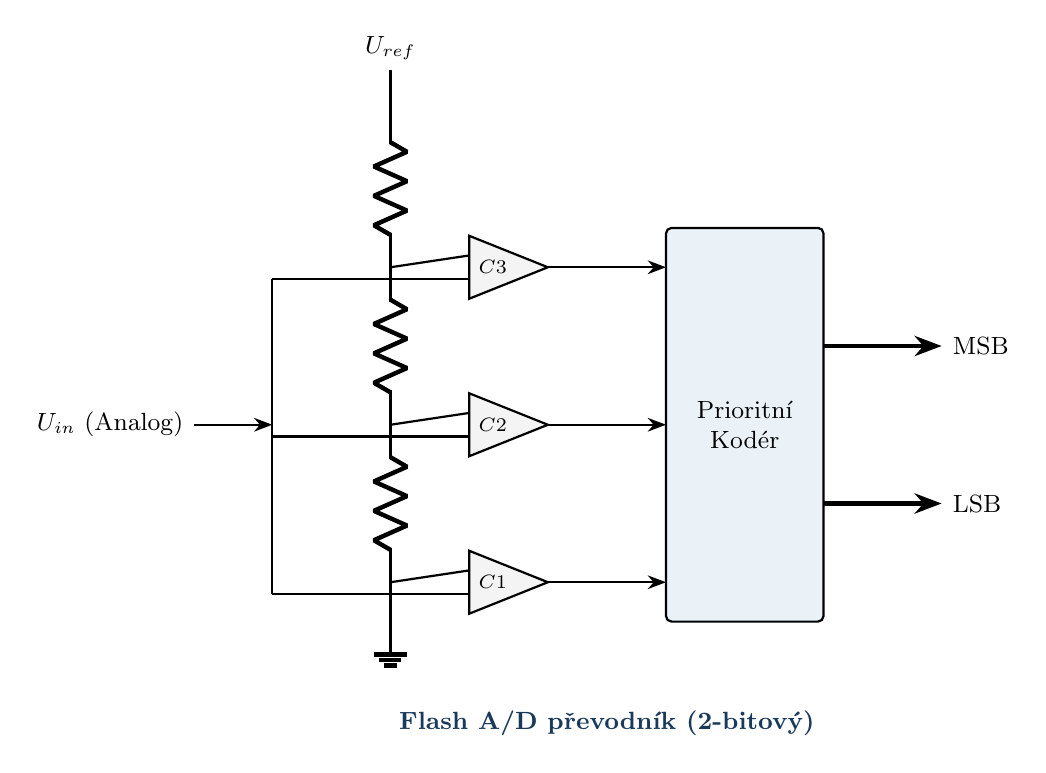
\begin{tikzpicture}[>=Stealth, font=\small, thick]
  % Odporový dělič (zvětšené rozestupy - z 1 dílku na 2 dílky)
  \draw (0,6.5) node[above] {$U_{ref}$} -- (0,6)
        to[R] (0,4)
        to[R] (0,2)
        to[R] (0,0)
        -- (0,-0.5) node[ground] {};

  % Komparátory
  \foreach \y/\n in {4/C3, 2/C2, 0/C1} {
    \draw[fill=lightgray] (1,\y-0.4) -- (1,\y+0.4) -- (2,\y) -- cycle;
    \node[font=\scriptsize] at (1.3,\y) {$\n$};
    \draw (0,\y) -- (1,\y+0.15); % Minus vstup
    \draw (-1.5,\y-0.15) -- (1,\y-0.15); % Plus vstup (společný analog. signál)
    \draw[->] (2,\y) -- (3.5,\y);
  }

  % Analogový vstup
  \draw (-1.5, -0.15) -- (-1.5, 3.85);
  \draw[<-] (-1.5, 2) -- (-2.5, 2) node[left] {$U_{in}$ (Analog)};

  % Prioritní kodér
  \draw[fill=lightblue, rounded corners=2pt] (3.5, -0.5) rectangle (5.5, 4.5);
  \node[align=center, text width=1.5cm] at (4.5,2) {Prioritní\\Kodér};

  % Digitální výstup
  \draw[->, line width=1.5pt] (5.5, 3) -- (7, 3) node[right] {MSB};
  \draw[->, line width=1.5pt] (5.5, 1) -- (7, 1) node[right] {LSB};

  \node[below=0.5cm, accent] at (2.75,-1) {\textbf{Flash A/D převodník (2-bitový)}};
\end{tikzpicture}
\end{center}

\subsubsection*{B) A/D převodník s postupnou aproximací (SAR)}
Je to nejlepší kompromis mezi rychlostí a složitostí (mikrokontroléry, zvukové karty).
\textbf{Princip (Hádání čísla):} Obsahuje D/A převodník a jeden komparátor. Logika se ptá: "Je napětí větší než polovina rozsahu?" D/A převodník vygeneruje polovinu, komparátor to porovná. Pokud ano, MSB = 1. Pak se ptá: "Je větší než 3/4 rozsahu?" atd.
Pro 10bitový převod potřebuje přesně 10 kroků (taktů hodin).

\subsubsection*{C) Integrační A/D převodník (Dual-slope)}
Nabíjí kondenzátor neznámým vstupním napětím po přesně danou dobu. Poté ho vybíjí známým referenčním napětím a měří čas, za jak dlouho se vybije k nule.
\textbf{Vlastnosti:} Je extrémně **pomalý** (desítky měření za sekundu), ale **obrovsky přesný** a ignoruje rušení ze sítě (50Hz).
\textbf{Použití:} Digitální multimetry (měřáky napětí a proudu).

\end{vysvetlenibox}

\end{document}d
